\graphicspath{ {Figures/Pileup/} }

\chapter{Analysis Results}

\begin{figure}[]
	\centering
	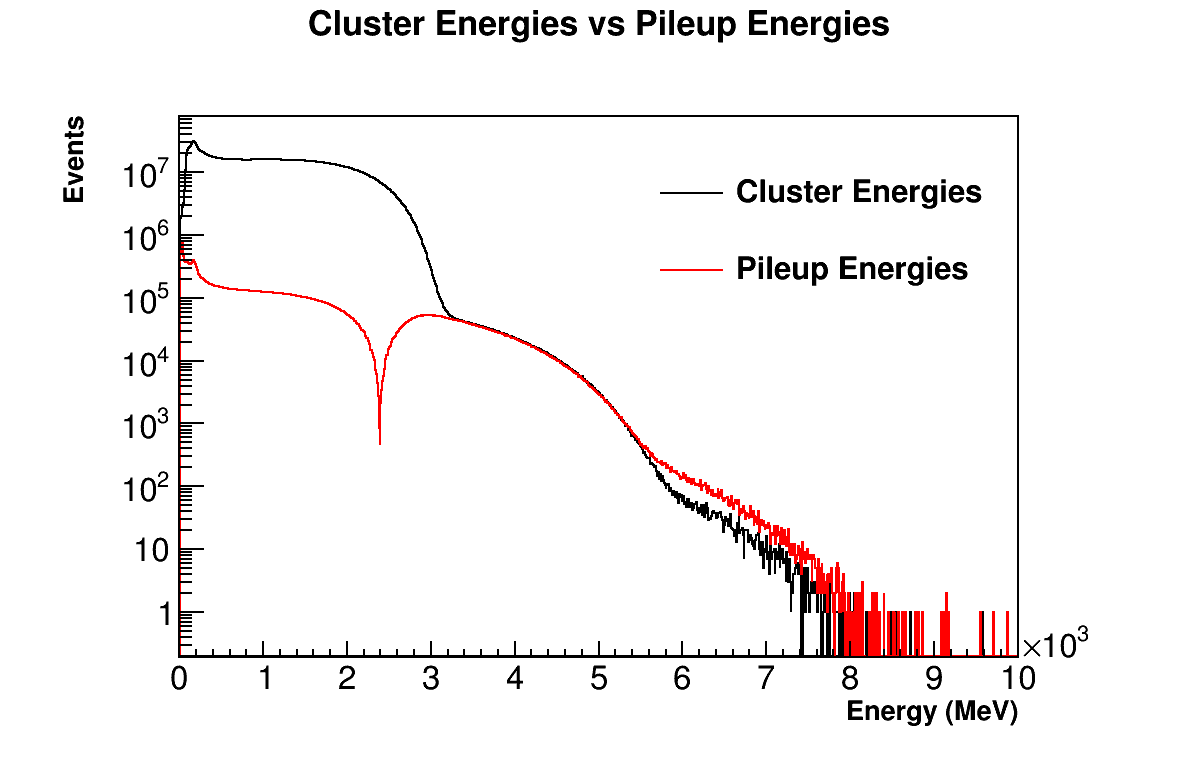
\includegraphics[width=\textwidth]{ClusterEnergiesVsPileupEnergies}
    \caption[ClusterEnergiesVsPileupEnergies]{Cluster energies in black are plotted vs pileup energies in red, for all calorimeters added together. At energies below about 2.4 GeV the pileup spectrum goes negative. In this plot the absolute value of the pileup energies is plotted, and a spike at about 2.4 GeV can be seen as a consequence of this. Due to the triplets and contamination in the pileup spectrum, the red and black curves can be seen to diverge at high energies.}    
    \label{fig:ClusterEnergiesVsPileupEnergies}
\end{figure}

\begin{figure}[]
\centering
    \begin{subfigure}[]{0.8\textwidth}
	    \centering
		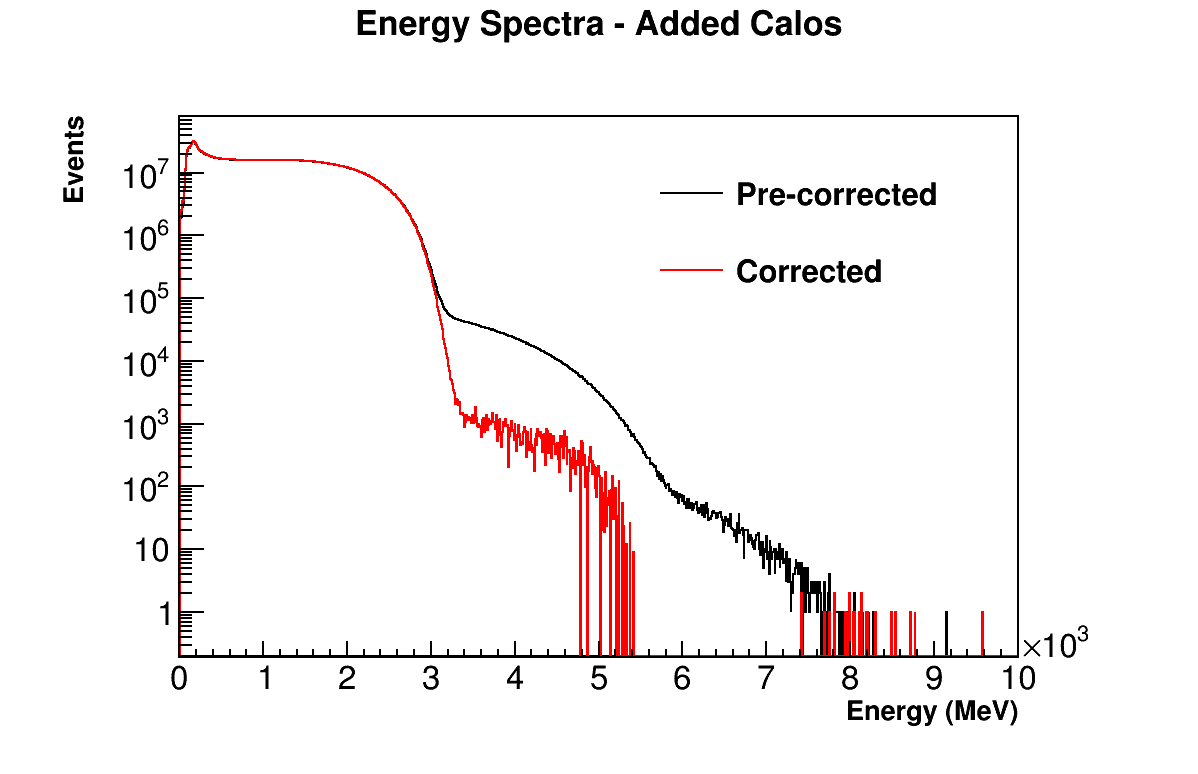
\includegraphics[width=\textwidth]{AddedEnergies}
	    \caption{Log scale - the corrected energy spectrum goes negative around 5 GeV.}
    \end{subfigure}% %you need this % here to add spacing between subfigures
    \vspace{1cm}
    \begin{subfigure}[]{0.8\textwidth}
	    \centering
		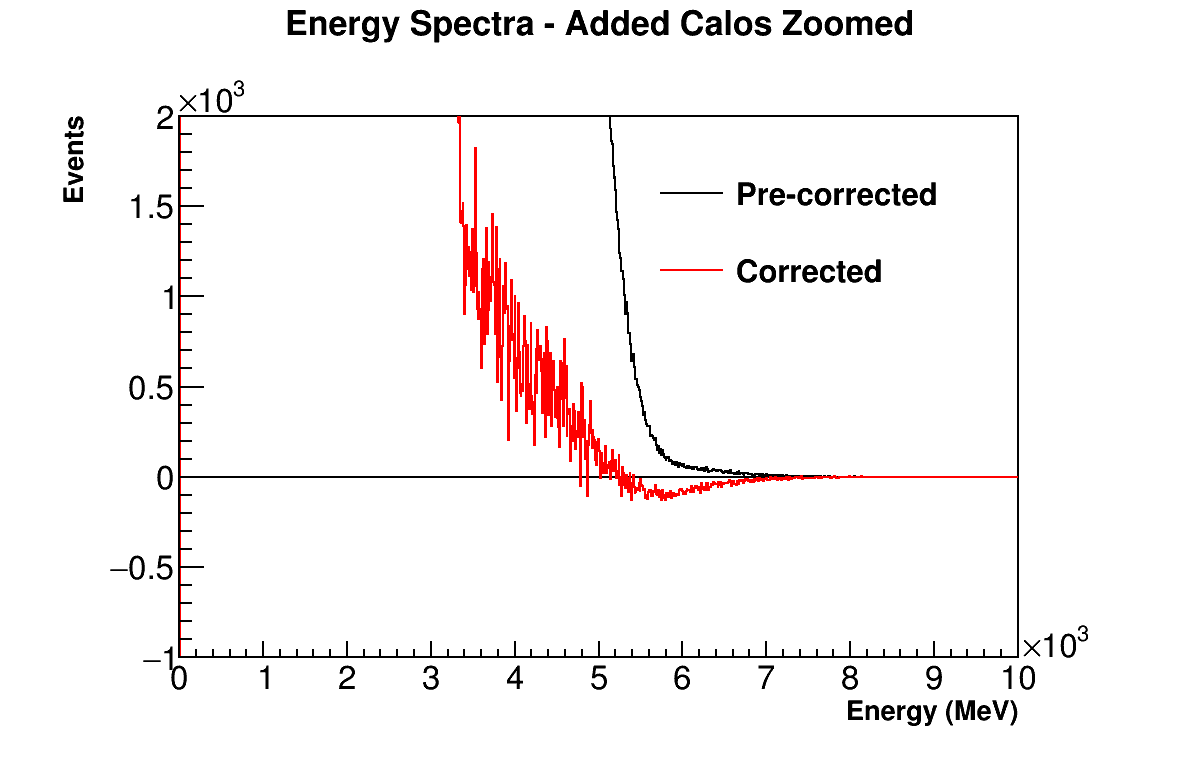
\includegraphics[width=\textwidth]{AddedEnergiesZoomed}
	    \caption{Linear scale - zoomed in to show the shape.}
    \end{subfigure}
\caption[AddedEnergies]{Plots for the pre-corrected and corrected energy spectra are shown, all calorimeters added together. Because the triplets and contamination are not accounted for, the corrected energy spectrum does not lie exacltly along zero.}
\label{fig:AddedEnergies}
\end{figure}

\begin{figure}[]
	\centering
	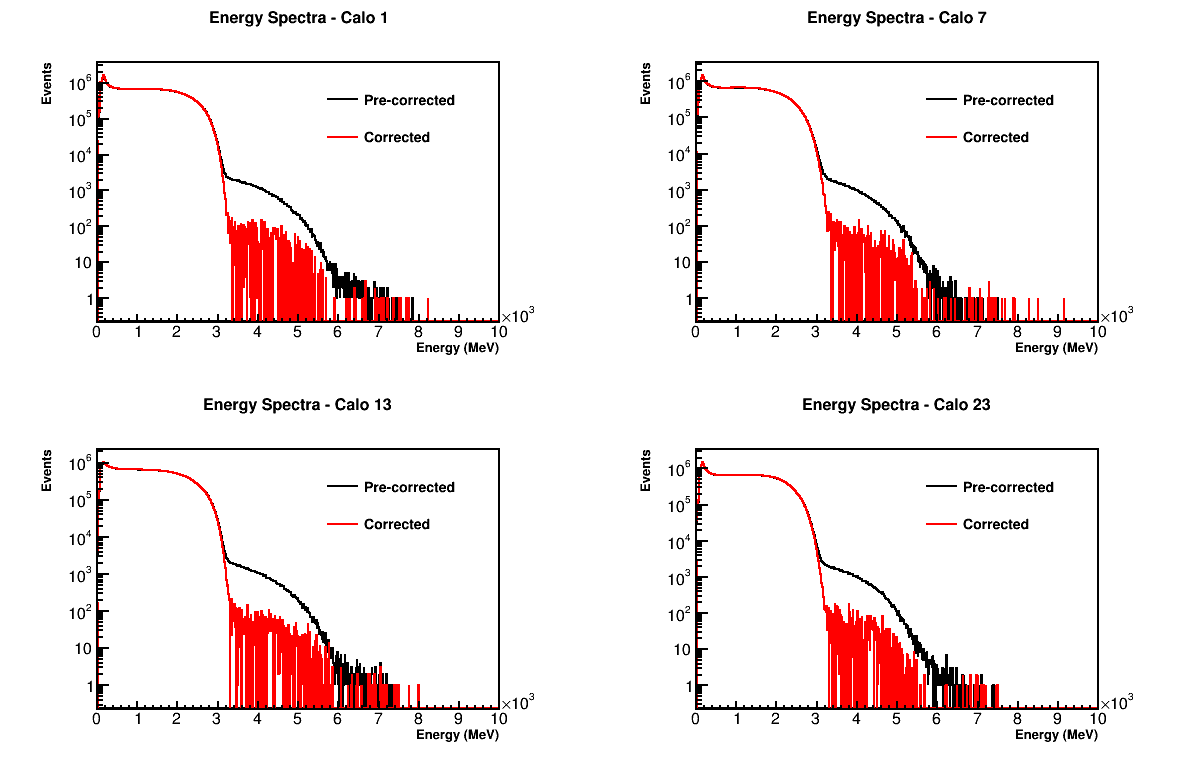
\includegraphics[width=\textwidth]{CaloEnergies}
    \caption[CaloEnergies]{Pre-corrected and corrected energy spectra for calorimeters 1, 7, 13, and 23 plotted on a log scale.}    
    \label{fig:CaloEnergies}
\end{figure}

\begin{figure}[]
	\centering
	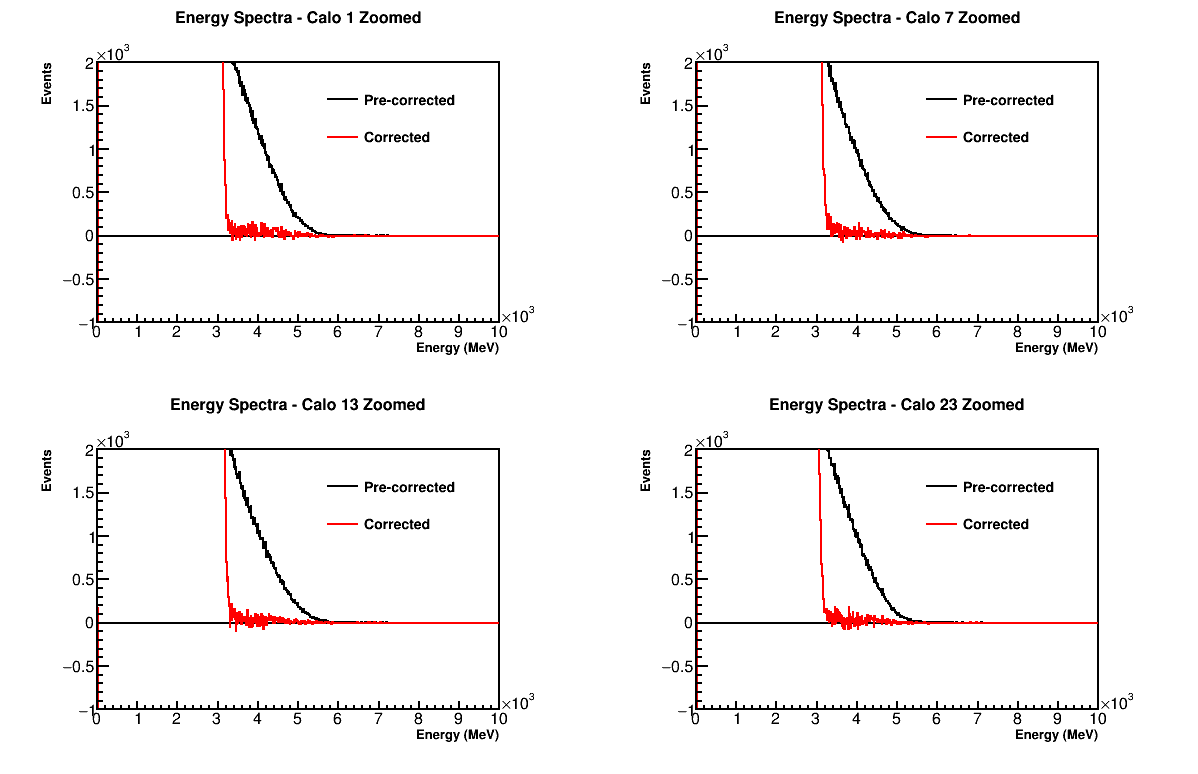
\includegraphics[width=\textwidth]{CaloEnergiesZoomed}
    \caption[CaloEnergiesZoomed]{Pre-corrected and corrected energy spectra for calorimeters 1, 7, 13, and 23 plotted on a linear scale and zoomed in.}    
    \label{fig:CaloEnergiesZoomed}
\end{figure}

\section{Pre-corrected and corrected energy and time spectra}

\section{6 Parameter Ratio Fit}


\section{Residual and FFT}




\section{Start time scans}


\section{Results vs calorimeter}



\section{Correlation matrix for fit parameters}



